\begin{figure}[t]
\centering
\pgfplotsset{compat=1.18}
% Harness colors
\definecolor{cNOOA}{RGB}{31,119,180}    % blue
\definecolor{cBASE}{RGB}{23,165,137}    % teal
\definecolor{cOC}{RGB}{230,126,34}      % orange
\definecolor{cPI}{RGB}{155,89,182}      % purple
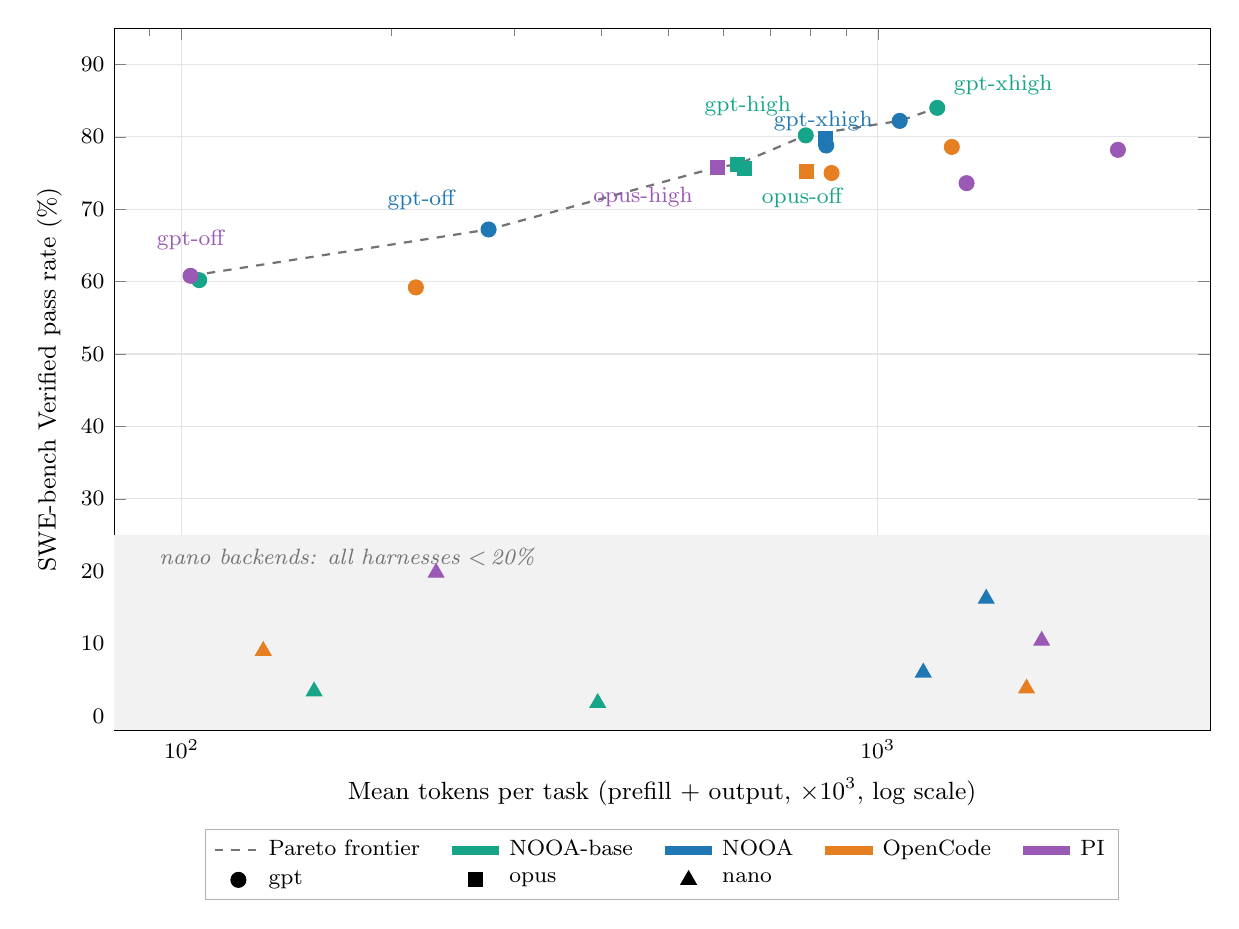
\begin{tikzpicture}
\begin{semilogxaxis}[
  width=15.5cm, height=10.5cm,
  xlabel={Mean tokens per task (prefill + output, $\times 10^3$, log scale)},
  ylabel={SWE-bench Verified pass rate (\%)},
  xmin=80, xmax=3000, ymin=-2, ymax=95,
  grid=major, grid style={black!10},
  legend cell align=left,
  legend style={
    at={(0.5,-0.14)}, anchor=north, legend columns=5,
    font=\footnotesize, draw=black!30,
    /tikz/every even column/.append style={column sep=8pt},
  },
  tick label style={font=\footnotesize}, label style={font=\small},
]
% ===== nano failure region =====
\fill[black!5] (axis cs:80,-2) rectangle (axis cs:3000,25);
\node[font=\footnotesize\itshape, black!55, anchor=west]
  at (axis cs:90,22) {nano backends: all harnesses $<$\,20\%};
% ===== Pareto frontier =====
\addplot[black!55, dashed, thick, mark=none] coordinates {
  (103,60.8) (276,67.2) (588,75.8) (629,76.2) (788,80.2) (1075,82.2) (1217,84.0)};
\addlegendentry{Pareto frontier}
% ===== data: color = harness, marker = backend family =====
% gpt = circle (*), opus = square, nano = triangle
\addplot[forget plot, only marks, mark=*,        mark size=2.7pt, cBASE] coordinates {(106,60.2) (788,80.2) (1217,84.0)};
\addplot[forget plot, only marks, mark=square*,  mark size=2.5pt, cBASE] coordinates {(629,76.2) (644,75.6)};
\addplot[forget plot, only marks, mark=triangle*,mark size=3.2pt, cBASE] coordinates {(155,3.4) (396,1.8)};
\addplot[forget plot, only marks, mark=*,        mark size=2.7pt, cNOOA] coordinates {(276,67.2) (843,78.8) (1075,82.2)};
\addplot[forget plot, only marks, mark=square*,  mark size=2.5pt, cNOOA] coordinates {(842,79.8)};
\addplot[forget plot, only marks, mark=triangle*,mark size=3.2pt, cNOOA] coordinates {(1162,6.0) (1431,16.2)};
\addplot[forget plot, only marks, mark=*,        mark size=2.7pt, cOC] coordinates {(217,59.2) (858,75.0) (1277,78.6)};
\addplot[forget plot, only marks, mark=square*,  mark size=2.5pt, cOC] coordinates {(791,75.2)};
\addplot[forget plot, only marks, mark=triangle*,mark size=3.2pt, cOC] coordinates {(131,9.0) (1635,3.8)};
\addplot[forget plot, only marks, mark=*,        mark size=2.7pt, cPI] coordinates {(103,60.8) (1341,73.6) (2212,78.2)};
\addplot[forget plot, only marks, mark=square*,  mark size=2.5pt, cPI] coordinates {(588,75.8)};
\addplot[forget plot, only marks, mark=triangle*,mark size=3.2pt, cPI] coordinates {(232,19.8) (1719,10.4)};
% ===== legend row 1: harness color swatches =====
\addlegendimage{cBASE, line width=3.2pt, mark=none}\addlegendentry{NOOA-base}
\addlegendimage{cNOOA, line width=3.2pt, mark=none}\addlegendentry{NOOA}
\addlegendimage{cOC,   line width=3.2pt, mark=none}\addlegendentry{OpenCode}
\addlegendimage{cPI,   line width=3.2pt, mark=none}\addlegendentry{PI}
% ===== legend row 2: backend shapes =====
\addlegendimage{only marks, mark=*,        mark size=2.7pt, black}\addlegendentry{gpt}
\addlegendimage{only marks, mark=square*,  mark size=2.5pt, black}\addlegendentry{opus}
\addlegendimage{only marks, mark=triangle*,mark size=3.2pt, black}\addlegendentry{nano}
% ===== frontier annotations (backend+effort; color = harness) =====
\node[font=\footnotesize, cPI,   anchor=south]      at (axis cs:103,63.0)  {gpt-off};
\node[font=\footnotesize, cNOOA, anchor=south east] at (axis cs:255,68.6)  {gpt-off};
\node[font=\footnotesize, cPI,   anchor=north east] at (axis cs:560,74.4)  {opus-high};
\node[font=\footnotesize, cBASE, anchor=north west] at (axis cs:660,74.2)  {opus-off};
\node[font=\footnotesize, cBASE, anchor=south east] at (axis cs:775,81.6)  {gpt-high};
\node[font=\footnotesize, cNOOA, anchor=east]       at (axis cs:1015,82.2) {gpt-xhigh};
\node[font=\footnotesize, cBASE, anchor=south west] at (axis cs:1245,84.4) {gpt-xhigh};
\end{semilogxaxis}
\end{tikzpicture}
\caption{SWE-Bench Verified score vs.\ per-task prefill+output token cost. Color encodes
harness; marker shape encodes backend family. Labels mark the Pareto-frontier configuration
at each cost tier.}
\end{figure}
